\subsubsection{Latency}
Latency is crucial when it comes to safety in platooning, because if message send over V2V from leading vehicle to following vehicle fails to come on time, it may result in crash. In the SARTRE project (\cite{Chan2012ProjectSARTRE}) they made a test of latency between Back office and Organisation assistant. Back office lies on the server and Organisation assistant is in the vehicle. It communicates with GPS and is sending vehicles’ GPS position to Back office through GSM/UMTS (V2I). Although these are not technologies we are using in V2V it is interesting to see how the latency differs in lower and higher traffic. The test was done on the road in the city as well as outside and in following times: 15:00-16:00 and 18:40–19:30.\par
% 
It can be observed that in the second case, the latency is higher due to the bigger traffic. This reminds us to bear in mind that the bigger the traffic is the bigger the latency and according to that some safety requirements must be set as well (for example: When the latency is higher than X milliseconds, minimum distance between vehicles must be Y meters). Nonetheless the latency should be kept as low as possible, because when using V2V to transmit data the latency may be a difference between safe stop of vehicle and crash.
% 
\begin{figure}[p]
    \centering
    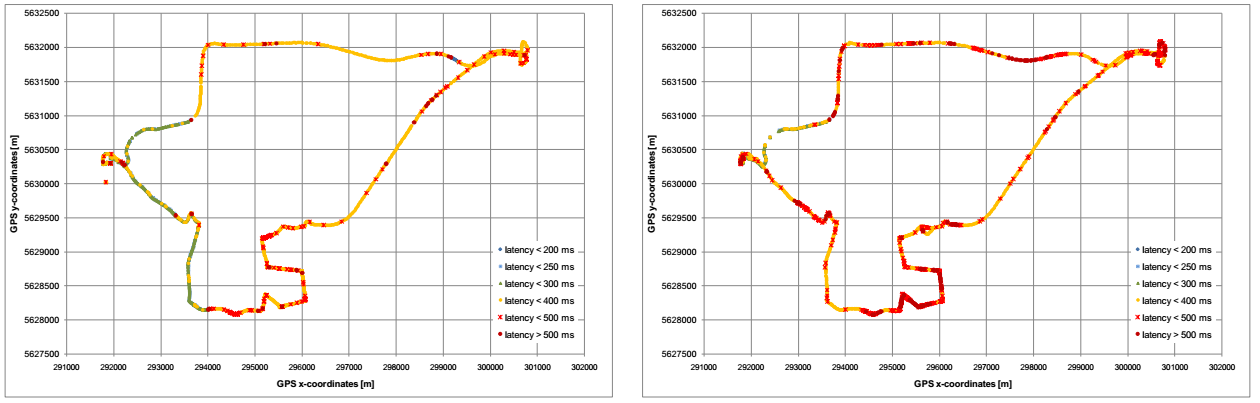
\includegraphics[width=.95\textwidth]{latency}
    \caption{Latency during testing in different day-times: Left 15:00-16:00, right 18:40-19:30. Taken from \cite[p. 24]{Chan2012ProjectSARTRE}}
    \label{fig:latency}
\end{figure}
% 